\documentclass[a4paper, 12pt]{article}

\newcommand{\languages}{french, english}

%%%%%%%%%%%%%%%%%%%

%%%%% Tools

\usepackage{comment}
\usepackage{lipsum}
\usepackage{xstring}

%%%%% Document

\usepackage[pdfusetitle]{hyperref}

\usepackage{geometry}
\geometry{paper=a4paper,top=2.5cm,bottom=2.5cm,right=2.5cm,left=2.5cm}

\usepackage{fancyhdr}
%\pagestyle{fancy}
%\fancyhead[L]{}
%\fancyhead[R]{\leftmark}
%\fancyfoot[C]{\thepage}
%\renewcommand{\headrulewidth}{0pt}

%%%%% Text

\usepackage[utf8]{inputenc}
\usepackage[T1]{fontenc}
\edef\restoreparindent{\parindent=\the\parindent\relax}
\usepackage[parfill]{parskip}
%\restoreparindent
\usepackage{csquotes}

\newlength{\mytextsize}
\makeatletter
\setlength{\mytextsize}{\f@size pt}
\makeatother

%%%%% Languages

\ifx\languages\undefined
	\usepackage[english]{babel}
\else
	\usepackage[\languages]{babel}
\fi

% english

\addto\captionsenglish{\def\figurename{Figure}}
\addto\captionsenglish{\def\tablename{Table}}

\def\st{\text{s.t.}}

% french

\frenchbsetup{StandardLists=true}

\addto\captionsfrench{\def\figurename{Figure}}
\addto\captionsfrench{\def\tablename{Table}}
\addto\captionsfrench{\def\proofname{Preuve}}

\def\tq{\text{t.q.}}
\def\cad{c.-à-d.}
\def\Cad{C.-à-d.}

%%%%% Styles

\usepackage[skip=\mytextsize]{caption}
\usepackage{float}
\usepackage{mdframed}
\usepackage{enumitem}
\usepackage{eurosym}
\usepackage{color}

\newcommand\caaption[1]{\caption{#1}\vspace{-1\mytextsize}}

%%%%% Mathematics

\usepackage{amsmath}
\usepackage{amssymb}
\usepackage{amsfonts}
\usepackage{bm}
\usepackage{esint}
\usepackage[makeroom]{cancel}

\newcommand{\fact}[1]{#1!}
\newcommand{\e}[1]{\mathbf{e}_{#1}}
\newcommand{\deriv}{\mathrm{d}}
\DeclareMathOperator{\tr}{tr}


%%%%% SI units

\usepackage[squaren,Gray,cdot]{SIunits}
\usepackage{sistyle}

\IfStrEq{\languagename}{french}{
	\SIdecimalsign{,}
}

%%%%% Chemistry

\usepackage[version=4]{mhchem}

%%%%% Table & Figure

\usepackage{subcaption}

\usepackage{array}
\usepackage{tabularx}
\usepackage{multirow}
\usepackage{multicol}
\newcolumntype{M}[1]{>{\centering\arraybackslash}m{#1}}
%\setlength\extrarowheight{0em}
\renewcommand{\arraystretch}{1.3}

\usepackage{pgfplots}
\usepackage{tikz}
\usetikzlibrary{shapes.geometric, positioning}
\usepackage{graphics}
\usepackage{graphicx}
\pgfplotsset{axis on top, compat = 1.3}

%%%%%% Theorems and Definitions

\usepackage{amsthm}
\usepackage{thmtools}

\def\lgthm{Theorem}
\def\lglem{Lemma}
\def\lgprop{Proposition}
\def\lgdefn{Definition}
\def\lghyp{Hypothesis}
\def\lgquest{Question}
\def\lgansw{Answer}
\def\lgexpl{Example}
\def\lgrmk{Remark}
\def\lgnote{Note}
\def\lgtip{Tip}

\IfStrEq{\languagename}{french}{
	\def\lgthm{Théorème}
	\def\lglem{Lemme}
	\def\lgprop{Proposition}
	\def\lgdefn{Définition}
	\def\lghyp{Hypothèse}
	\def\lgquest{Question}
	\def\lgansw{Réponse}
	\def\lgexpl{Exemple}
	\def\lgrmk{Remarque}
	\def\lgnote{Note}
	\def\lgtip{Conseil}
}

\theoremstyle{plain}
\newtheorem{thm}{\lgthm}[section]
\newtheorem{lem}{\lglem}[section]
\newtheorem{prop}{\lgprop}[section]

\theoremstyle{definition}
\newtheorem{defn}{\lgdefn}[section]
\newtheorem{hyp}{\lghyp}[section]
\newtheorem{quest}{\lgquest}[]

\declaretheorem[
name=\lgansw,
qed={\lower-0.3ex\hbox{$\triangle$}},
within=quest
]{answ}

\declaretheorem[
name=\lgexpl,
qed={\lower-0.3ex\hbox{$\triangle$}},
within=section
]{expl}

\theoremstyle{remark}
\newtheorem*{rmk}{\lgrmk}
\newtheorem*{note}{\lgnote}
\newtheorem*{tip}{\lgtip}

\begingroup
\makeatletter
\@for\theoremstyle:=definition,remark,plain\do{%
	\expandafter\g@addto@macro\csname th@\theoremstyle\endcsname{%
		\addtolength\thm@preskip\parskip
	}%
}
\endgroup

%%%% Others

\renewcommand{\qedsymbol}{$\blacksquare$}

\newcommand{\mytableofcontents}{
	\newpage
	\pagenumbering{roman}
	\tableofcontents
	\newpage
	\pagenumbering{arabic}
}

%%%%%%%%%%%%%%%%%%%
\makeatletter
\AtBeginDocument{
	\hypersetup{
		pdftitle={\@title},
		pdfauthor={Maxime Meurisse, Valentin Vermeylen},
		pdfkeywords={maxime, meurisse, valentin, vermeylen, artificial, intelligence, info8006, pacman, bayes, filter, latex, document},
		pdfproducer={LaTeX document},
		pdfcreator={Document generated with pdflatex}
	}
}

%%%%%%%%%%%%%%%%%%%

\title{Introduction to artificial intelligence\\Pacman - Reasoning over time}
\author{Maxime \textsc{Meurisse} (20161278)\and Valentin \textsc{Vermeylen} (20162864)}
\date{Academic year 2018-2019}

%%%%%%%%%%%%%%%%%%%

\begin{document}
    % ---------- Title page ---------- %
    \maketitle
    
    
    % ---------- Discussion ---------- %
    \section{Discussion of the results}
    \label{sec:discussion}
    In order to discuss the convergence of each case, the entropy was calculated\footnote{The code is not in the submitted file as to not mix up the analysis and the actual implementation of the filter, but consists in the sum described below.}. This is computed, at each iteration, on the basis of all probabilities (but only the nonzero ones will affect the entropy) of the possible positions of the ghost via the formula:
    \begin{equation}
        H_2\left (X\right ) = -\sum_{i=1}^n P_i\log_2 P_i
    \end{equation}
    We chose to work in a binary logarithm as the entropy then represents the number of bits necessary to encode the information (for example, in our case, an entropy of \num{3} for a ghost would mean \(2^3 = 8\) possible (non-zero probability) positions for this ghost).\par
    For each case (several combinations of values of the parameters \(w\) and \(p\)), the entropy was calculated at each iteration. Measurements were taken for \num{100}, \num{200} and \num{500} iterations. All results are shown in the section \ref{sec:figures}\footnote{All graphs are in vectorial quality and can thus be zoomed in without loss of quality.}.\par
    We only computed the entropy for one ghost in each situation as they do not interact with one another and the Bayes filtering for each one is therefore independent. Furthermore, each graph shows the mean entropy of \num{5} games to avoid special cases, although the shape does not vary much between the plot of the means and the plot of a single game.\par
    \subsection{Observations}
    In each case, we see that the entropy oscillates. This oscillation always ends up being bounded by a value lower than \(\log_2((2w+1)^2)\). Therefore, and as can be seen during the execution, some positions end up having a zero probability in the possible nonzero probability square defined by the sensor model. The fact that we do not tend to a unique value can be easily understood by watching a game. For example, the algorithm will provide some high probability positions, sometimes only one (the entropy being \num{0} as \(\log(1) = 0\) and it is the only nonzero probability) but will eventually separate into equiprobable positions as east is no longer a possible action.\par 
    As a general rule, we see that  the lesser \(p\), the slower the convergence and the greater the upper bound on the entropy. When \(p = 0\), we see that we have the biggest entropy of all cases, and for all \(w\).\par
    That is easily understood as a greater \(p\) means less incertitude about the whereabouts of the ghost, as it will most certainly turn east if it can.\par 
    As \(w\) increases, the entropy increases, as can be seen on the vertical axis when \(w\) goes from \num{1} to \num{3}, and from \num{3} to \num{5}. However, on figure \ref{fig:200_p0}, we have almost no difference in the bounds of \(w = 5\) and \(w = 7\). That is probably because, as the square of evidence grows larger, \num{2} successive evidence can be quite far from one another, which means that the number of non-zero probability elements does not increases too much. Moreover, more walls may get included in the computations, and our transition model gives them a probability of \num{0}, as described in the second section.\par
    We also see that some games require up to \num{40} iterations to converge and, for some big \(w\) and low \(p\), we may go up to \num{200}. That was more easily seen in the graphs of one game instead of the plots of the means, although the general tendency is still to be seen (great decrease in entropy in the first \num{10} to \num{20} moves and stabilization not long after). Convergence appears as the oscillations become quite bounded, and manifests itself visually as a checker pattern.
    \paragraph{Remark} As expected, a \(w\) of \num{0} produces an entropy of \num{0} as the sensor model always provides the exact location of the ghost with probability \num{1}.
    
    
    % ---------- Improvement ---------- %
    \section{Filter improvement}
    The results discussed in the section \ref{sec:discussion} could be improved. Indeed, our agent could take into account the fact that he receives measures for ghosts that are not always physically possible, such as a position on a wall, for example. We only focused on that kind of improvement, as was asked by the statement. However, smoothing could be applied to the previous state matrix to have better approximations.\par
    Currently, the probability that a ghost is on a position \(x\) is calculated using the following formula:
    \begin{equation}
        P\left (\bm{X}_{t+1}|\bm{e}_{1:t+1}\right ) = \alpha P\left (\bm{e}_{t+1}|\bm{X}_{t+1}\right )\sum_{\bm{X_t}}P\left (\bm{X}_{t+1}|\bm{X}_{t}\right )P\left (\bm{X}_{t}|\bm{e}_{1:t}\right )
    \end{equation}
    We can try to improve each term of this equation by taking into account these non physically possible measures.
    
    \subsection{The sonar sensor model}
    The sonar sensor model is represented by the term \(P\left (\bm{e}_{t+1}|\bm{X}_{t+1}\right )\).\par
    To improve it, we could sample the evidence received if we had more evidence at each time step and the one received did not make sense with the model (moving in a wall, teleporting in an enclosed space,...), or give a zero probability to the ghost being in a wall on the \(W\times W\) zone. That means that the prior (represented by the term \(P\left (\bm{X}_{t}|\bm{e}_{1:t}\right )\)) would only provide a uniform distribution over the legal squares and \num{0} on the walls. Probabilities are therefore increased on actual legal squares. That is the solution to use in our case where we cannot sample (we have only one observation per time step).
    
    \subsection{The transition model}
    The transition model is represented by the term \(P\left (\bm{X}_{t+1}|\bm{X}_{t}\right )\).\par
    To improve it, we \textbf{already} implemented the following policy: if a ghost tries to enter a wall, the probability associated with that action is \num{0}, and if it is in a wall, it has no way of getting out as that situation is only possible if we received a noised estimation of that position. It cannot be in a wall. The probability associated to that case (getting out of a wall to a legal case) is therefore \num{0}.\par
    Probabilities of a ghost being in a wall are therefore non \num{0} only when we receive the first uniform prior.
    \paragraph{Remark} We could consider that a ghost can leave a wall if it is in it, but the algorithm would converge more slowly.
    
    
    \appendix
    % ---------- Figures ---------- %
    \section{Figures}
    \label{sec:figures}
    \begin{figure}[!ht]
        \centering
        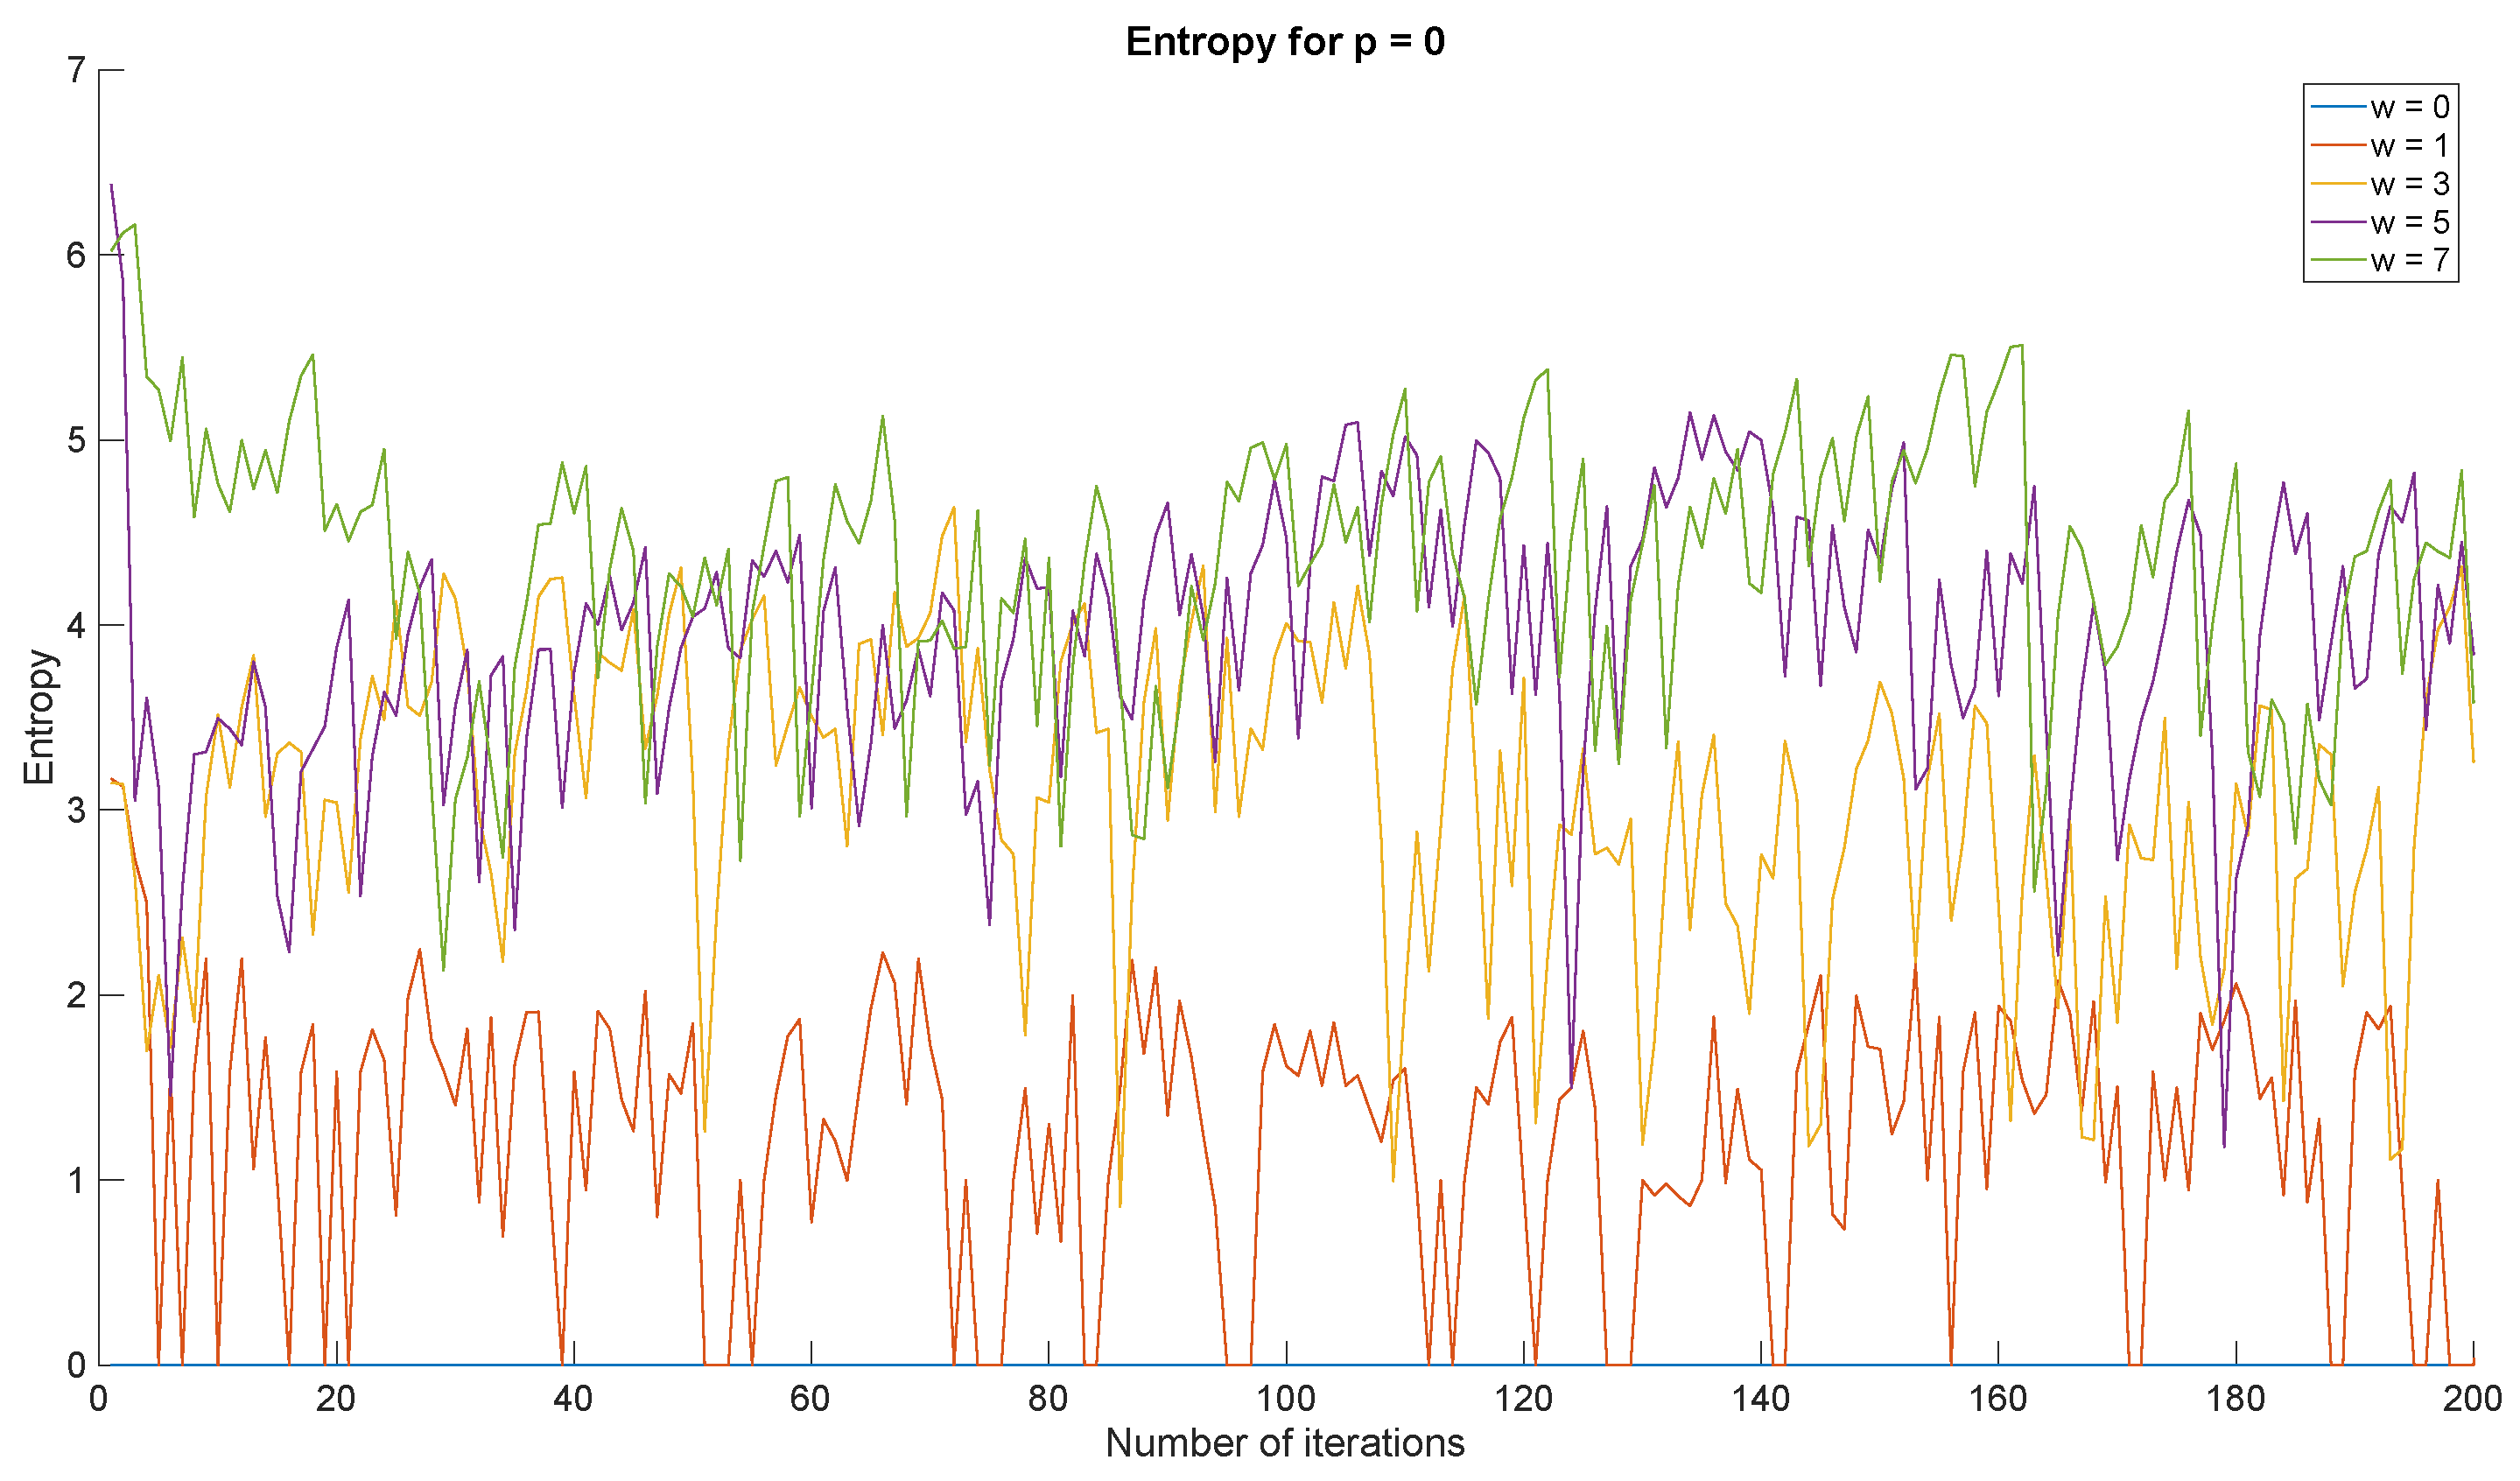
\includegraphics[width=0.9\textwidth]{resources/pdf/200/p0.pdf}
        \caption{Entropy for \(p = 0\) and \num{5} values of \(w\).}
        \label{fig:200_p0}
    \end{figure}
    \begin{figure}[!ht]
        \centering
        \includegraphics[width=\textwidth]{resources/pdf/compacted/1_bis.pdf}
        \caption{Entropy values for several combinations of the parameters \(w\) (\num{1}, \num{3}, \num{5}) and \(p\) (\num{0.3}, \num{0.5}, \num{0.7}) over several iterations (\num{100} and \num{500}).}
    \end{figure}
\end{document}
